\documentclass[10pt,a4paper]{report}

% Packages
\usepackage[a4paper,margin=0.9in]{geometry} % reduce margins
\usepackage{setspace}
\usepackage{titlesec}
\usepackage{hyperref}
\usepackage{graphicx} % for images
\usepackage{caption}  % better caption control
\usepackage{lipsum}   % for dummy text (remove later)
\usepackage{enumitem}
\usepackage{amssymb} % for \checkmark symbol
\usepackage{fancyhdr}
\pagestyle{fancy}
\fancyhead[L]{CS202 Lab Assignment 2 Report}
\fancyhead[R]{Shardul Junagade, Ridham Patel}
\fancyfoot[C]{\thepage}
\usepackage{xcolor}
\newcommand{\command}[1]{\texttt{\textcolor{blue}{#1}}}
\usepackage{float} % put this in the preamble

\setlength{\parindent}{0pt}
\setlength{\parskip}{0.6em}

% Remove figure numbering
\captionsetup[figure]{labelformat=empty}

% Customize section/chapter fonts
\titleformat{\chapter}[block]{\huge\bfseries}{}{0pt}{}
\titleformat{\section}{\Large\bfseries}{\thesection}{0.4em}{} 
\titleformat{\subsection}{\large\bfseries}{\thesubsection}{0.4em}{} 

% Define custom command for images with optional caption
\usepackage{xparse}
\NewDocumentCommand{\insertimage}{O{0.8\textwidth} m o}{%
    \begin{center}
        \includegraphics[width=#1]{#2}%
        \IfValueT{#3}{\\\captionof{figure}{#3}}%
    \end{center}
}


% Front Page Info
\title{\Huge Assignment-2 \\[0.5cm] \LARGE Software Tools and Techniques for CSE}
\author{\Large Shardul Junagade (23110297) \\[0.2cm] \Large Repository: \href{https://github.com/ShardulJunagade/cs202-stt}{cs202-stt}}
\date{\large \today}

\begin{document}

% Front Page
\maketitle
\newpage

% Table of Contents
\tableofcontents
\newpage

% ---------- Lab 7 ----------
\chapter{Lab Assignment 7: Reaching Definitions Analyzer for C Programs}

\textbf{Course:} CS202 -- Software Tools and Techniques for CSE\\
\textbf{Lab Topic:} Reaching Definitions Analyzer for C Programs\\
\textbf{Name:} Shardul Junagade\\
\textbf{Roll Number:} 23110297\\
\textbf{Date:} 15th September 2025

\vspace{0.5em}
\textbf{Repository Link(s):} \href{https://github.com/ShardulJunagade/cs202-stt/tree/main/lab7/}{\texttt{lab7/}} \space (runner: \href{https://github.com/ShardulJunagade/cs202-stt/tree/main/lab7/run\_analysis.py}{\texttt{lab7/run\_analysis.py}}, code: \href{https://github.com/ShardulJunagade/cs202-stt/tree/main/lab7/analyzer/}{\texttt{lab7/analyzer/}})


\section{Introduction, Setup, and Tools}

\subsection{Introduction}
I implemented an intraprocedural analyzer that constructed Control Flow Graphs (CFGs) for single-file C programs and ran Reaching Definitions analysis on top of them. I created DOT/PNG CFGs, per-iteration data-flow tables, a definitions index, an ambiguity report, and basic metrics including cyclomatic complexity.

\subsection{Environment and Tools}
\begin{itemize}[itemsep=0em, topsep=0pt]
    \item OS: Windows 11; Terminal: PowerShell 7
    \item Python: 3.13.7
    \item Required tools: Graphviz (for \texttt{dot}), Matplotlib (for plots)
    \item Editor: VS Code Insiders
\end{itemize}

\insertimage[0.8\textwidth]{../images/lab7/1.png}[Environment Details]

\section{Program Corpus}

I selected three single-file C programs (200--300 LOC each) that had conditionals, loops, and multiple reassignments, as required. I chose programs that were self-contained to avoid interprocedural complexity.

\begin{itemize}[itemsep=0em, topsep=0pt]
    \item Program 1: \href{https://github.com/ShardulJunagade/cs202-stt/tree/main/lab7/programs/inventory_tracker.c}{\texttt{inventory\_tracker.c}} -- tracked stock levels with multiple conditionals and loop-based updates; good mix of assignments.
    \item Program 2: \href{https://github.com/ShardulJunagade/cs202-stt/tree/main/lab7/programs/student_performance.c}{\texttt{student\_performance.c}} -- computed aggregates with branch-heavy logic around grading thresholds.
    \item Program 3: \href{https://github.com/ShardulJunagade/cs202-stt/tree/main/lab7/programs/weather_simulator.c}{\texttt{weather\_simulator.c}} -- iterative simulation with nested condition checks and loop-carried updates.
\end{itemize}

\insertimage[0.7\textwidth]{../images/lab7/2.png}[\texttt{lab7/programs} folder snapshot]

\section{Approach and Implementation}

\subsection{Parsing and Cleaning -- \href{https://github.com/ShardulJunagade/cs202-stt/tree/main/lab7/analyzer/c_parser.py}{\texttt{analyzer/c\_parser.py}}}
\begin{itemize}[itemsep=0em, topsep=0pt]
    \item I first read the source and stripped preprocessor lines and comments:
    Removed \texttt{\#...} lines and both \texttt{/* ... */} and \texttt{// ...} comments.
    \insertimage[0.8\textwidth]{../images/lab7/3.png}[Code snippet -- \texttt{strip\_preprocessor\_and\_comments}]
    \item Extracted only the body of \texttt{main()} and tracked its starting line so later line numbers stayed meaningful.
    \insertimage[0.8\textwidth]{../images/lab7/4.png}[Code snippet -- \texttt{extract\_main\_function\_source}]
    \item I kept it deliberately simple; this worked fine for my inputs but wasn’t a full C parser.
\end{itemize}

\subsection{Basic Blocks and CFG Construction -- \href{https://github.com/ShardulJunagade/cs202-stt/tree/main/lab7/analyzer/cfg_builder.py}{\texttt{analyzer/cfg\_builder.py}}}
I used leader-based basic block detection per the instructions given in the lab document. Blocks were labeled \texttt{B0}, \texttt{B1}, \ldots{} and I added edges for sequential flow, conditionals, and simple loops:
\begin{itemize}[itemsep=0em, topsep=0pt]
    \item Leaders: first statement, the condition of \texttt{if/else if/else/while/for}, the statement after a branch/jump.
    \insertimage[0.8\textwidth]{../images/lab7/5.png}[Code snippet -- \texttt{\_find\_leaders}]
    \item Edges: for \texttt{if} I added true/false; for \texttt{while/for} I added back-edges from body to condition.
    \item Jumps like \texttt{return/break/continue} terminated flow for that block.
    \insertimage[0.8\textwidth]{../images/lab7/6.png}[Code snippet -- \texttt{\_build\_edges\_from\_blocks}]
\end{itemize}

I exported a DOT graph for each program, and rendered it to PNG if \texttt{dot} was in PATH using Graphviz. Following in the code snippet shows the export and rendering logic.

\insertimage[0.8\textwidth]{../images/lab7/6_dot.png}[Code snippet -- DOT export and PNG rendering]

% \insertimage[0.7\textwidth]{../images/lab7/cfg.png}[Sample CFG (Preview)]
\noindent
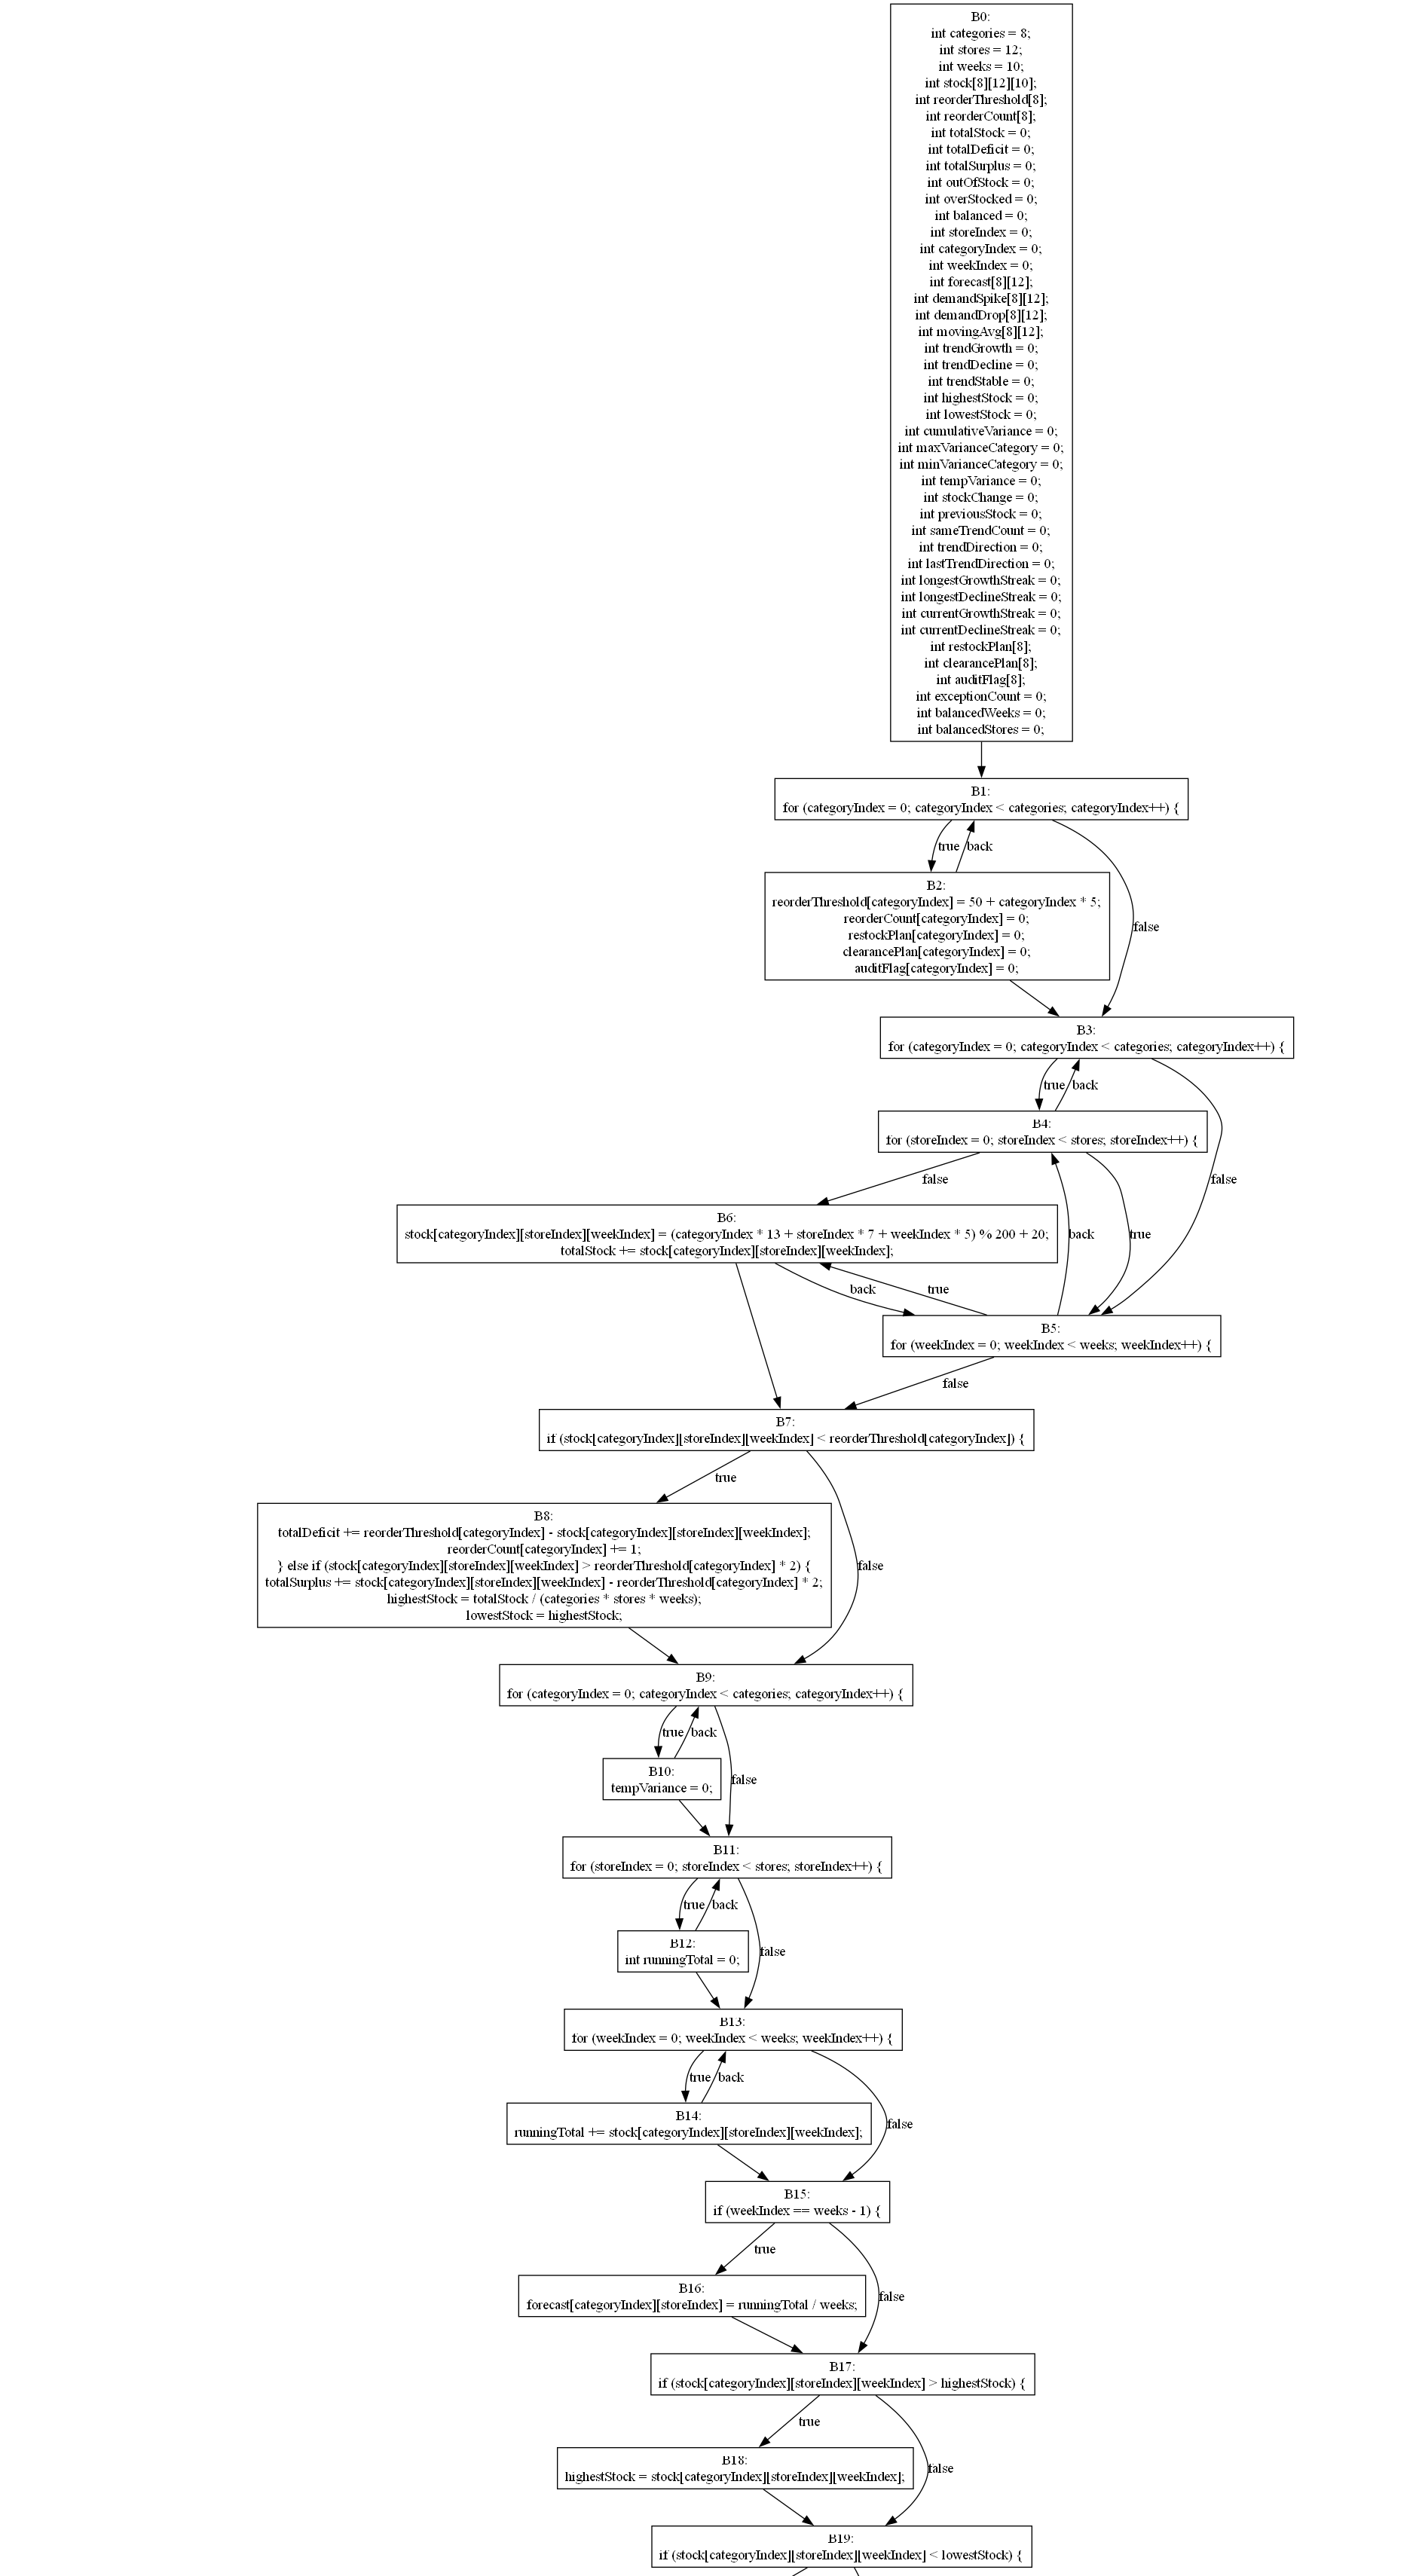
\includegraphics[width=0.33\textwidth]{../images/lab7/cfg1.png}%
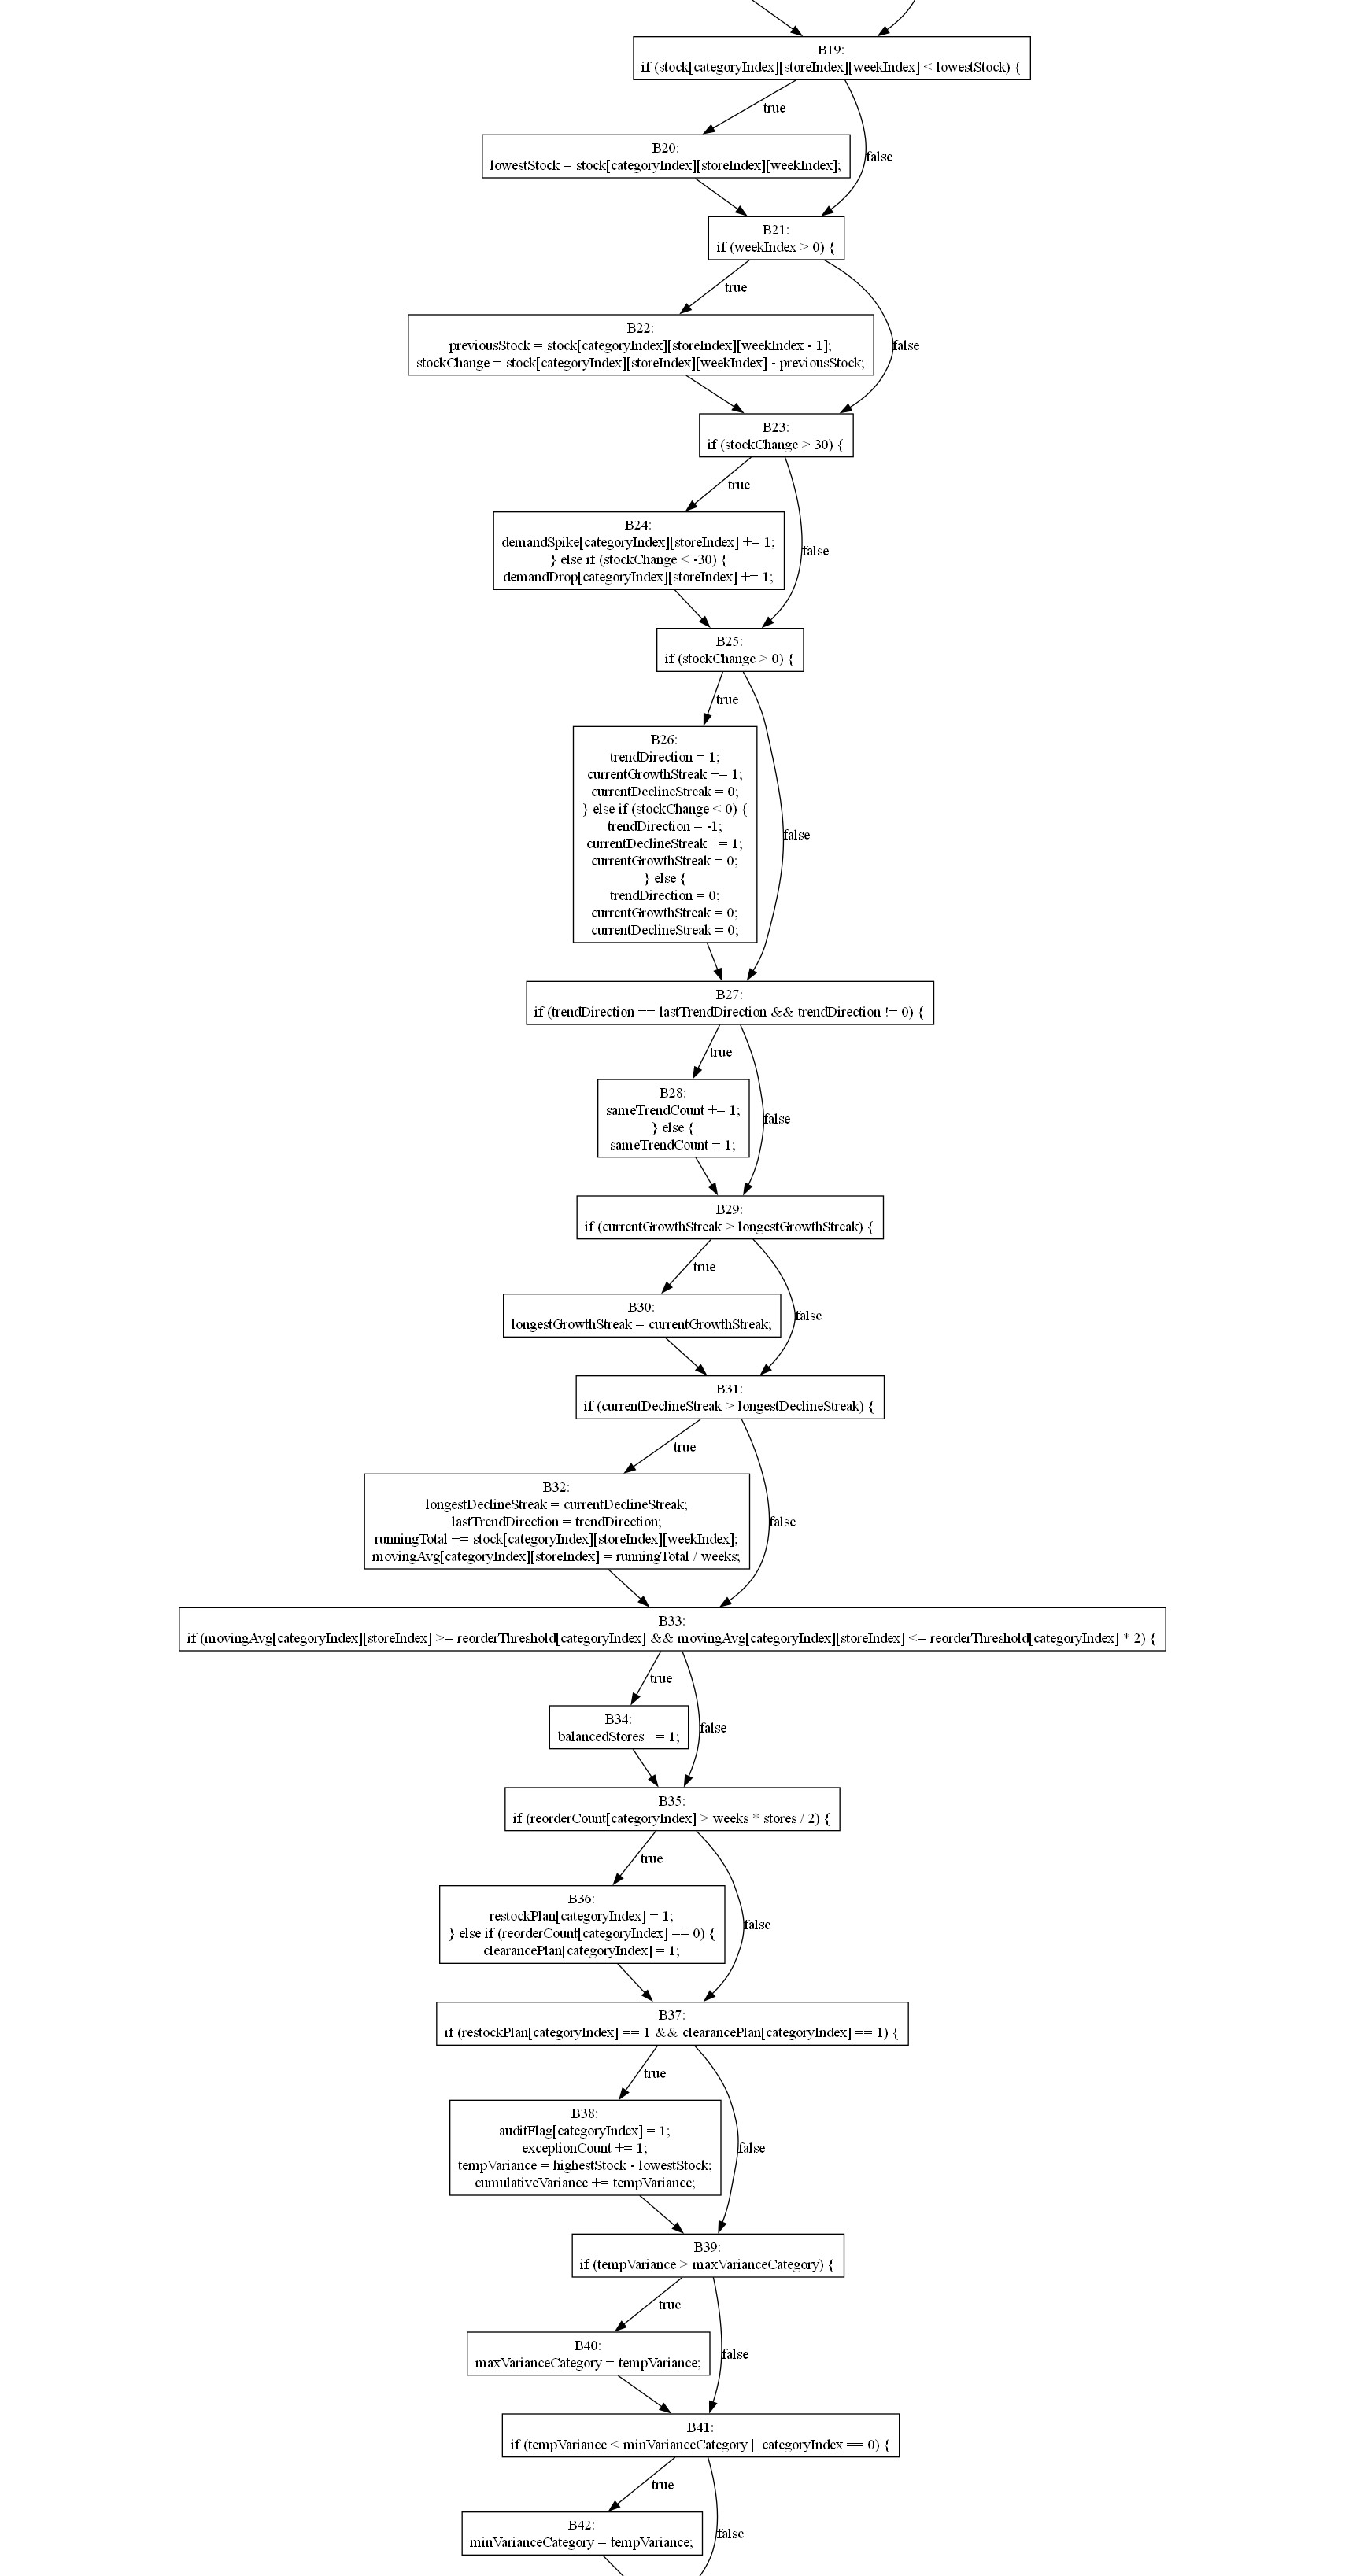
\includegraphics[width=0.33\textwidth]{../images/lab7/cfg2.png}%
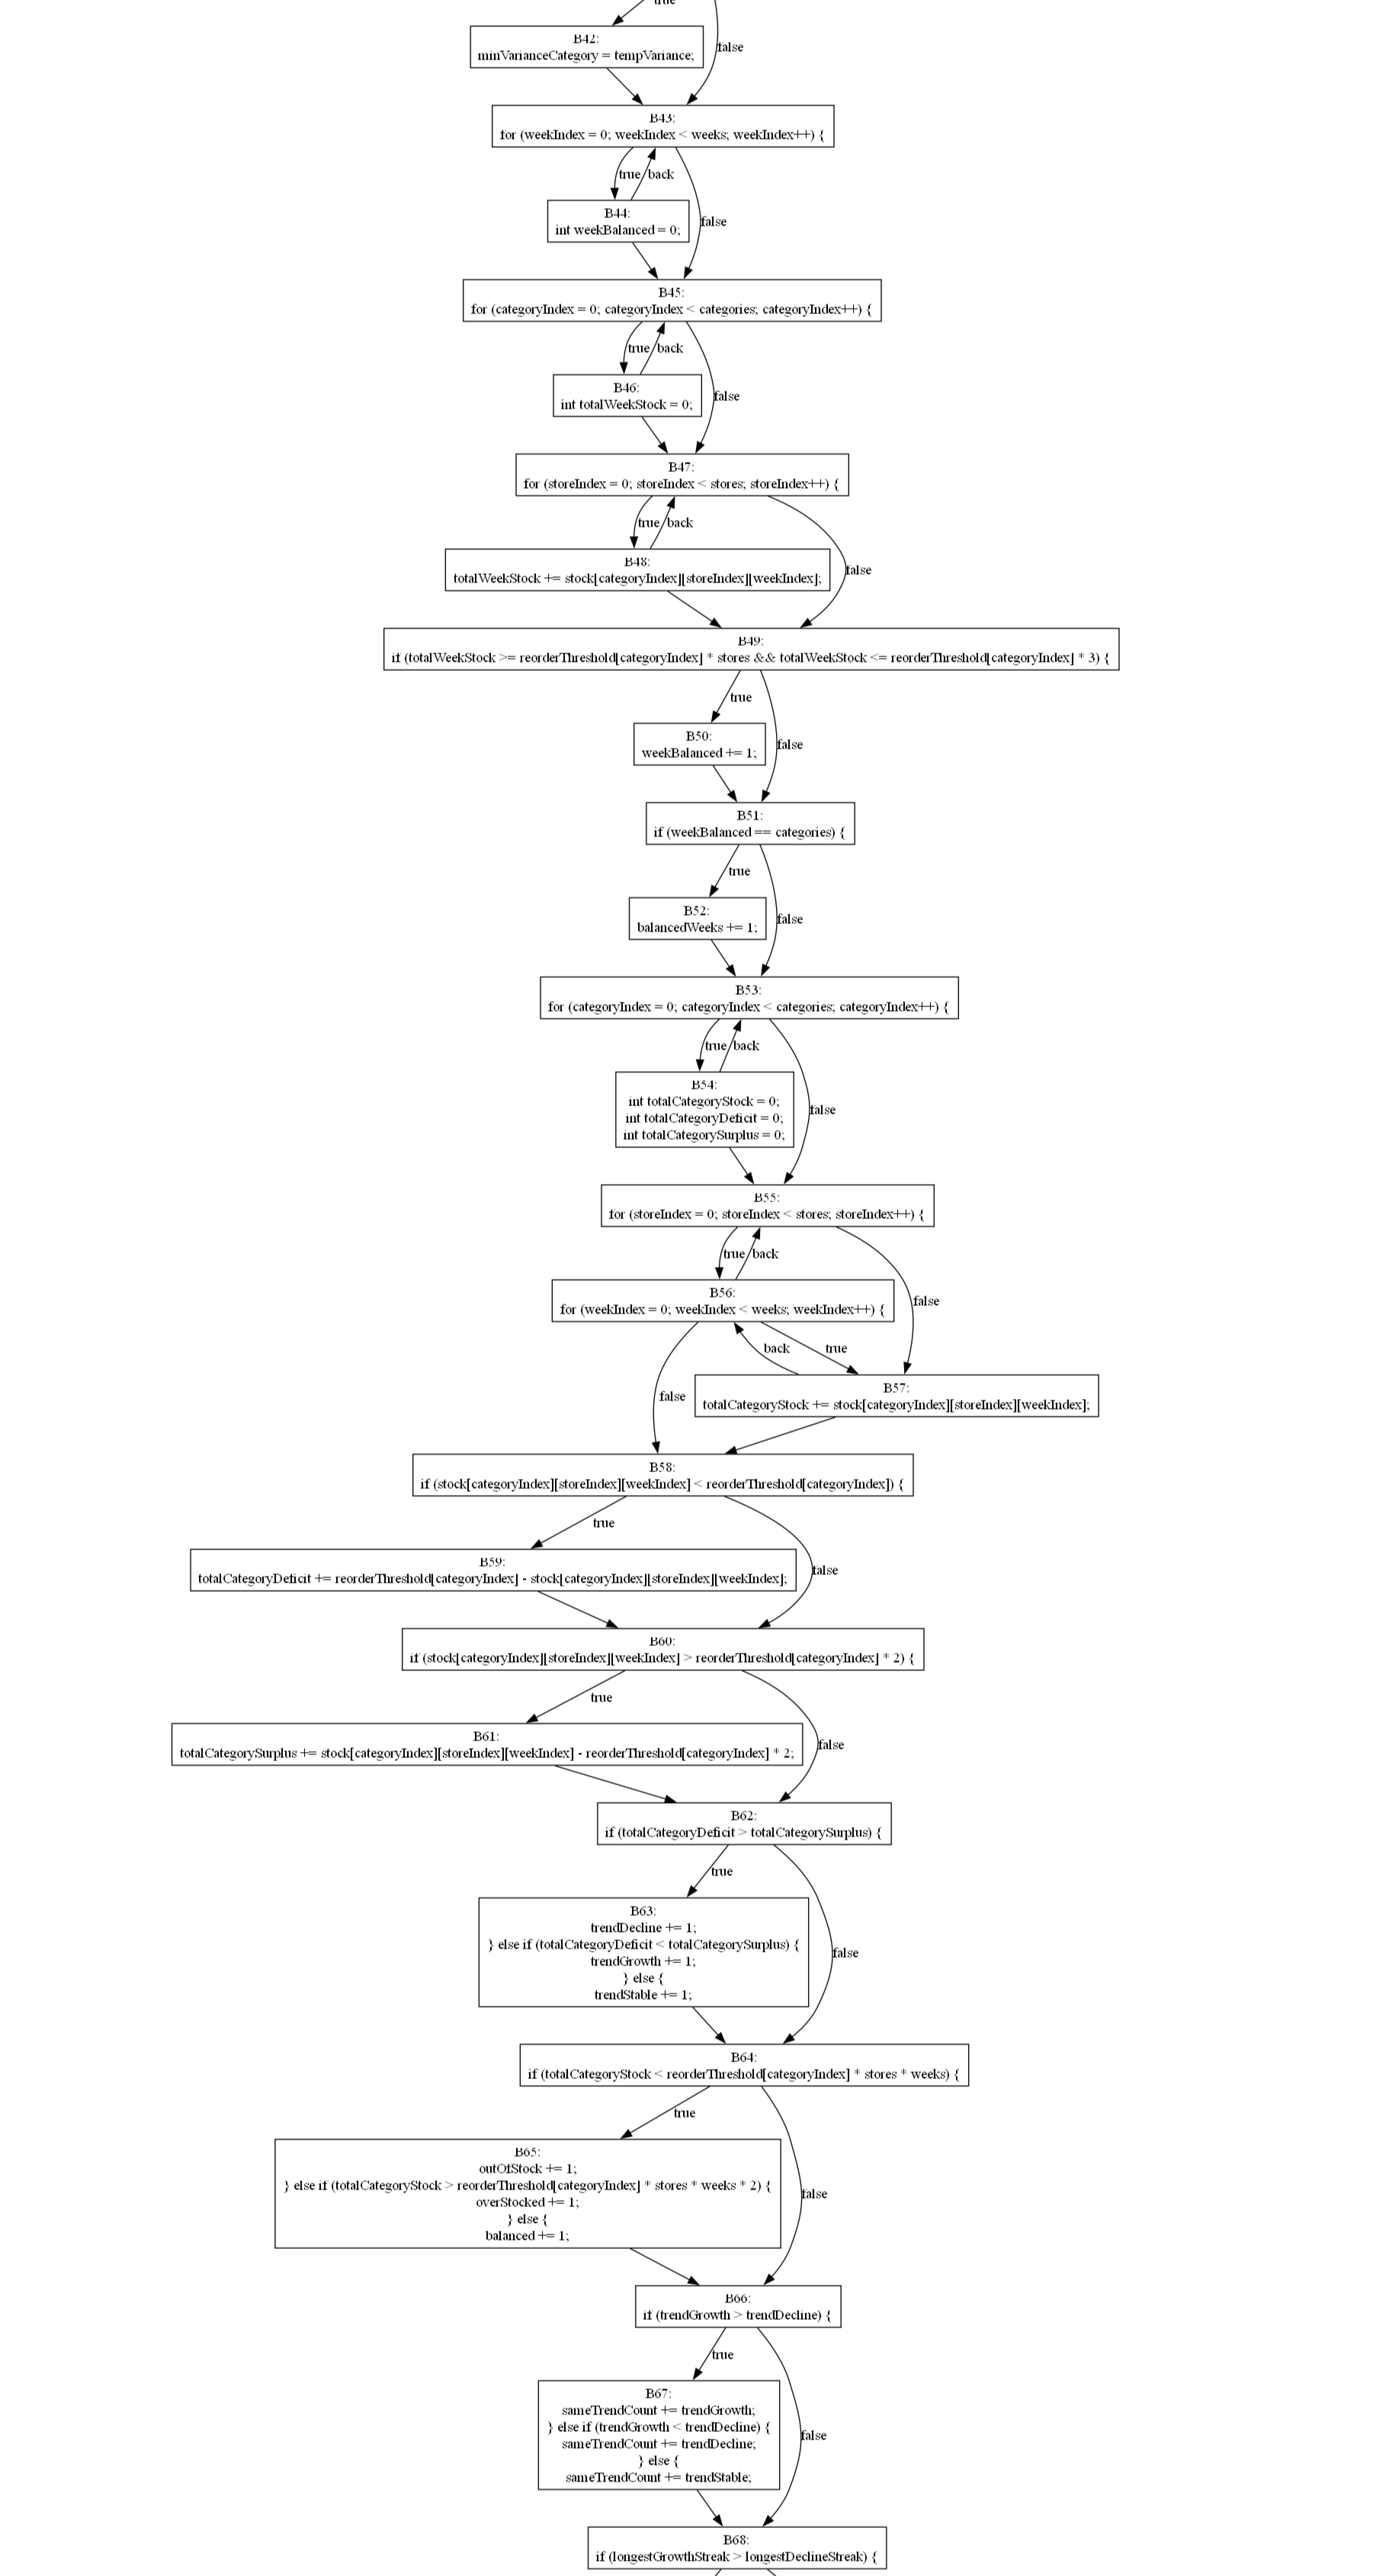
\includegraphics[width=0.33\textwidth]{../images/lab7/cfg3.png}

Link to sample CFG: \href{https://github.com/ShardulJunagade/cs202-stt/tree/main/lab7/output/inventory_tracker/cfg.png}{inventory\_tracker CFG PNG} \space (too big to embed here)


\subsection{Definition Extraction -- \href{https://github.com/ShardulJunagade/cs202-stt/tree/main/lab7/analyzer/cfg_builder.py}{\texttt{analyzer/cfg\_builder.py}}}
For each statement, I extracted defined variables and created unique definition IDs (\texttt{D1}, \texttt{D2}, \ldots):
\begin{itemize}[itemsep=0em, topsep=0pt]
    \item Handled declarations like \texttt{int x = 0;}, \texttt{int x, y;} and simple assignments including compound ops like \texttt{+=}.
    \item Counted increments/decrements as definitions.
    \item Stored each definition with statement text, block ID, and line number.
\end{itemize}

I wrote a Markdown table (\texttt{definitions.md}) for quick reference. Following is the code snippet for the same:

\insertimage[0.8\textwidth]{../images/lab7/7.png}[Code snippet -- \texttt{\_extract\_defined\_variables\_from\_text}]

\insertimage[0.7\textwidth]{../images/lab7/8.png}[\texttt{definitions.md} preview]

\subsection{gen/kill Sets per Block -- \href{https://github.com/ShardulJunagade/cs202-stt/tree/main/lab7/analyzer/cfg_builder.py}{\texttt{analyzer/cfg\_builder.py}}}

I computed \texttt{gen[B]} and \texttt{kill[B]} for each block:
\begin{itemize}[itemsep=0em, topsep=0pt]
    \item \textbf{gen[B] (generated definitions):} All definitions that are created inside block B.
    \item \textbf{kill[B] (killed definitions):} All other definitions of the same variables that exist outside block B.
\end{itemize}
I computed \texttt{gen[B]} and \texttt{kill[B]} as the latest definitions per variable within a block, in program order. The code snippet below shows the implementation (\texttt{compute\_gen\_kill\_sets}).

\insertimage[0.65\textwidth]{../images/lab7/9.png}[Code snippet -- \texttt{\_compute\_gen\_kill\_sets}]


\subsection{Reaching Definitions (Data-Flow) -- \href{https://github.com/ShardulJunagade/cs202-stt/tree/main/lab7/analyzer/dataflow.py}{\texttt{analyzer/dataflow.py}}}
I implemented the standard forward data-flow equations (\texttt{analyzer/dataflow.py}):
\begin{itemize}[itemsep=0em, topsep=0pt]
    \item $in[B] = \bigcup out[P]$ over predecessors $P$
    \item $out[B] = gen[B] \cup (in[B] - kill[B])$
\end{itemize}

I iterated until the sets stopped changing. I recorded every iteration as a snapshot and wrote a Markdown table with \texttt{gen/kill/in/out} for each block per iteration. Following is the snippet for the iteration logic:

\insertimage[0.65\textwidth]{../images/lab7/10.png}[Code snippet -- \texttt{compute\_reaching\_definitions}]

\insertimage[0.8\textwidth]{../images/lab7/11.png}[\texttt{reaching\_definitions\_iterations.md} preview]

\subsection{Ambiguity Detection -- \href{https://github.com/ShardulJunagade/cs202-stt/tree/main/lab7/analyzer/dataflow.py}{\texttt{analyzer/dataflow.py}}}
After convergence, I flagged blocks where a variable had more than one reaching definition in \texttt{in[B]} (\texttt{find\_ambiguous\_variables}). I summarized them with the corresponding statements for context (\texttt{ambiguity.md}).

\insertimage[0.8\textwidth]{../images/lab7/12.png}[Code snippet -- \texttt{find\_ambiguous\_variables}]

\insertimage[0.8\textwidth]{../images/lab7/13.png}[\texttt{ambiguity.md} preview]

\subsection{Runner and Outputs}
The runner (\href{https://github.com/ShardulJunagade/cs202-stt/tree/main/lab7/run_analysis.py}{\texttt{lab7/run\_analysis.py}}) processed all \texttt{.c} files in \texttt{lab7/programs/} and wrote per-program outputs to \texttt{lab7/output/\textless program\_name\textgreater{}/}:
\begin{itemize}[itemsep=0em, topsep=0pt]
    \item \texttt{cfg.dot} (+ \texttt{cfg.png} if Graphviz was available)
    \item \texttt{definitions.md}
    \item \texttt{reaching\_definitions\_iterations.md}
    \item \texttt{ambiguity.md}
    \item \texttt{summary.json} (nodes, edges, CC)
\end{itemize}

\insertimage[0.8\textwidth]{../images/lab7/14.png}[Code snippet -- Runner invoking analysis and writing outputs]

\insertimage[0.8\textwidth]{../images/lab7/15.png}[Terminal Output]

I also wrote code to generate an overall \href{https://github.com/ShardulJunagade/cs202-stt/tree/main/lab7/output/metrics_summary.md}{\texttt{metrics\_summary.md}} and, if Matplotlib was available, a bar chart \href{https://github.com/ShardulJunagade/cs202-stt/tree/main/lab7/output/cyclomatic_complexity.png}{\texttt{cyclomatic\_complexity.png}} at \texttt{lab7/output/}.

\insertimage[0.8\textwidth]{../images/lab7/16.png}[Code snippet -- Metrics summary generation]

\insertimage[0.8\textwidth]{../images/lab7/17.png}[\texttt{metrics\_summary.md} preview]

\insertimage[0.8\textwidth]{../images/lab7/18_cyclomatic_complexity.png}[Cyclomatic Complexity Chart]

\section{Results}

I am attaching links to key outputs for each program below because they are too large to embed here.

\subsection{CFG and Metrics}

Links to CFG PNGs for each program:
\begin{itemize}[itemsep=0em, topsep=0pt]
    \item \href{https://github.com/ShardulJunagade/cs202-stt/tree/main/lab7/output/inventory_tracker/cfg.png}{inventory\_tracker}
    \item \href{https://github.com/ShardulJunagade/cs202-stt/tree/main/lab7/output/student_performance/cfg.png}{student\_performance}
    \item \href{https://github.com/ShardulJunagade/cs202-stt/tree/main/lab7/output/weather_simulator/cfg.png}{weather\_simulator}
\end{itemize}

For each program, I reported the number of nodes (basic blocks), edges, and cyclomatic complexity \texttt{CC = E - N + 2}. The chart helped me compare CCs across the three programs at a glance.

Actual metrics from my run (\texttt{lab7/output/metrics\_summary.md}):

\begin{table}[H]
\centering
\begin{tabular}{|l|l|l|l|}
\hline
Program & Nodes (N) & Edges (E) & Cyclomatic Complexity (CC) \\
\hline
inventory\_tracker & 76 & 126 & 52 \\
student\_performance & 59 & 98 & 41 \\
weather\_simulator & 76 & 120 & 46 \\
\hline
\end{tabular}
\end{table}

\subsection{Reaching Definitions Tables}
I skimmed early iterations to sanity-check propagation, and I confirmed convergence when tables stopped changing. I then used the final snapshot to interpret variable reachability.

Links to final iteration tables for each program:
\begin{itemize}[itemsep=0em, topsep=0pt]
    \item \href{https://github.com/ShardulJunagade/cs202-stt/tree/main/lab7/output/inventory_tracker/reaching_definitions_iterations.md}{inventory\_tracker}
    \item \href{https://github.com/ShardulJunagade/cs202-stt/tree/main/lab7/output/student_performance/reaching_definitions_iterations.md}{student\_performance}
    \item \href{https://github.com/ShardulJunagade/cs202-stt/tree/main/lab7/output/weather_simulator/reaching_definitions_iterations.md}{weather\_simulator}
\end{itemize}

\subsection{Ambiguity Highlights}
I listed a few examples where variables had multiple reaching definitions at a program point and explained why (e.g., different branches or loop-carried definitions).

Links to detailed ambiguity tables for each program:
\begin{itemize}[itemsep=0em, topsep=0pt]
    \item \href{https://github.com/ShardulJunagade/cs202-stt/tree/main/lab7/output/inventory_tracker/ambiguity.md}{inventory\_tracker}
    \item \href{https://github.com/ShardulJunagade/cs202-stt/tree/main/lab7/output/student_performance/ambiguity.md}{student\_performance}
    \item \href{https://github.com/ShardulJunagade/cs202-stt/tree/main/lab7/output/weather_simulator/ambiguity.md}{weather\_simulator}
\end{itemize}

\section{Discussion and Reflection}

\subsection{Challenges}
I faced a few challenges while implementing the analyzer. Getting the leader-based heuristics to behave well across nested conditionals, chained \texttt{else if} constructs, and loops required careful compromises. I deliberately kept the reconstruction simple, which worked for my programs but isn’t a full CFG reconstructor. I also had to filter out syntactic noise early (like standalone braces and empty statements) to keep basic blocks clean. Finally, I ensured that Graphviz was installed and on PATH by updating the environment variables on my Windows machine.

\subsection{What I Learned}
This assignment gave me a hands-on understanding of how control-flow and data-flow analyses fit together in practice. Building CFGs forced me to think in terms of basic blocks, leaders, and edges for branches and loops. I got a better understanding of data-flow analysis by defining \texttt{gen/kill} precisely and then iterating the reaching definitions equations $in[B] = \bigcup out[P]$ and $out[B] = gen[B] \cup (in[B] - kill[B])$. Tracing iteration snapshots helped me verify convergence and understand why certain variables had multiple reaching definitions at a point (ambiguity due to branches or loop-carried updates). Overall, I learned how to move from raw C source to CFGs, to \texttt{gen/kill} sets, to stable reaching definitions.

\subsection{Further Improvements}
\begin{itemize}[itemsep=0em, topsep=0pt]
    \item Swap the lightweight parsing for a proper C front-end (e.g., \texttt{pycparser}) to cover more syntax and nesting reliably.
    \item Refine CFG edges for more complex constructs and labels.
    \item Add unit tests for tricky statements (declarations with pointers/arrays, compound statements).
\end{itemize}

\newpage
\section{References}
\begin{itemize}[itemsep=0em, topsep=0pt]
    \item Lecture 7 slides: \href{https://drive.google.com/file/d/1cMLqFTzRJcpvq8iTEL4XV0K9BclsALzE/view}{here}
    \item Lab Assignment 7 document: \href{https://drive.google.com/file/d/1x6MDZ6e2PJ0MFn6u2U8NPzMxtcuhOy2t/view}{here}
    \item Data-flow analysis: \url{https://en.wikipedia.org/wiki/Data-flow_analysis}
    \item Graphviz: \url{https://graphviz.org/}
    \item PyGraphviz: \url{https://pygraphviz.github.io/}
\end{itemize}


\end{document}
